This section presents an inter-annotator agreement (IAA) section that aims to gain a better understanding of the annotation process of negation cues in texts related to the vaccination debate using the e-Host annotation tool. The purpose of this section is to compare, analyze, and quantify the annotations made by different annotators and to identify sources of disagreement among them, with the ultimate goal of improving the final classification.

To ensure consistency, the annotation process follows the guidelines provided by Morante et al. \cite{morante2011annotation}. Each member of the group independently annotates the same corpus of texts, which contains a mix of pro and anti-vaccination opinions from various sources, including official sources such as the National Health Service UK, as well as independent publications like the National Vaccine Information Center and Natural News.

The annotation guidelines provide possible negation cues for each part of speech and offer examples on how to determine the scope of the negation. They also include instructions on how to separate the negation scope from the rest of the phrase based on a simple grammatical analysis, which involves reformulating the phrase to test whether a part of it belongs to the scope or not. Specific rules on the separation of scope based on the part of speech that was negated are provided to minimize the annotator's bias. Special constructions such as questions and imperatives are also included in the guidelines, as well as examples of false negations and non-existing scope, to avoid expected mistakes.

Overall, this section aims to provide insights into the annotation process of negation cues and how it could impact the final classification. By comparing, analyzing, and quantifying the annotations made by different annotators, this section contributes to the understanding of the sources of disagreement and helps identify areas for improvement in the annotation process.
% All annotations were added to our \href{https://github.com/Sergi095/Applied-Text-Mining-VU-Course-2023-}{GitHub Repository}

\subsection*{Inter-Annotator Agreement Analysis}
As part of our investigation into the annotation process and its impact on the final classification, an inter-annotator agreement (IAA) analysis was conducted. In this section, we present the results of the IAA analysis and discuss the sources of disagreement among the annotators.

Each member of the group independently annotated a set of 12 texts following the guidelines provided by Morante et al. \cite{morante2011annotation}, which offered detailed instructions on how to identify negation cues and determine their scope. The purpose of the IAA analysis was to compare, analyze, and quantify the annotations made by different annotators and to identify sources of disagreement among them.

\begin{figure}[!h]
\begin{center}
  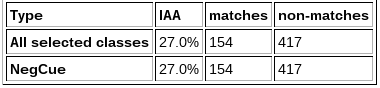
\includegraphics[width=0.6\textwidth]{Plots and results/4way.png}
  \caption{4-way IAA result}
  \label{fig:4way}
\end{center}  
\end{figure}

The results of the IAA analysis were obtained by comparing the annotations made by each member of the group. Figure \ref{fig:Pairwise agreement} shows the pair-wise agreement scores obtained from the analysis. We conducted an error analysis to systematically identify and explain the sources of disagreement among annotators. The analysis was based on a random sample of errors, and patterns were identified and illustrated with examples.

\begin{figure}[!h]
  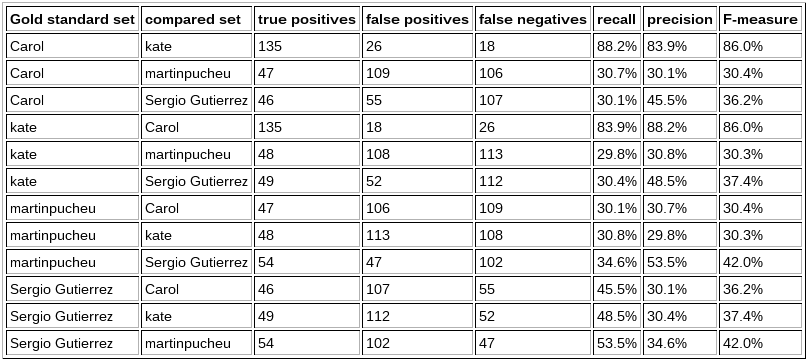
\includegraphics[width=\linewidth]{Plots and results/pairwise.png}
  \caption{Pair-wise agreement}
  \label{fig:Pairwise agreement}
\end{figure}

The results of the analysis revealed that human error and a lack of alignment between the text versions used for annotation were the main sources of disagreements among annotators. Specifically, disagreements arose when annotators failed to highlight the entire word or phrase, instead only highlighting part of it. For example, with words like "unclear", "unprotected", and "unpublished", some annotators highlighted the complete word, while others only highlighted the prefix "un". Similarly, with the word "don't", some annotators only highlighted the contraction, while others did the complete word.

To address these sources of disagreement, we suggest implementing a more thorough training process for the annotators, which could include a detailed review of the guidelines and examples, as well as further practice sessions. Moreover, we suggest that the guidelines could be further expanded to cover more examples of negation cues in different contexts to reduce ambiguity. Additionally, post-processing the annotations to annotate some obvious negations missed by the classifier would also help to improve the overall agreement scores, as shown in Figure \ref{fig:4way}.


To sum up, this section provided insights into the annotation process of negation cues. The inter-annotator agreement analysis helped to identify the sources of disagreement among the annotators and highlighted the need for more thorough training to reduce ambiguity. The results also emphasized the importance of post-processing the annotations to improve the overall agreement scores.
